\documentclass[internal]{../../classes/nervtech-research}

\nervsetup{
  company={NervTech},
  project={Node v0},
  document={Research Notes},
  subtitle={Problem framing, goal association, assumptions and associated research papers},
  docid={NT-N-CR-000},
  revision={A},
  status={Exploratory Draft},
  author={NervTech Research},
  owner={Robotics Systems Engineering},
  date={2026-08-22},
  stage={Preliminary Research},
  question={Which cycloidal speed reducer architecture will fulfill NT-N-G1 and NT-N-G7?},
  keywords={integrated actuator, mechanical design, cycloidal speed reducer, robotics, research notes},
  abstract={This document collates and analyses multiple research papers and notes for fulfilling Node v0 design goals in relation to cycloidal speed reducer design. Its intended purpose is to isolate observations, assumptions, risks, and design direction before committing to a detailed technical design.}
}

\begin{document}
\maketitle
\tableofcontents
\newpage

\section{Research Snapshot}
\researchsnapshot
{Build a cycloidal speed reducer to maximise torque density and minimise backlash, making it easy to integrate with existing motor housing architectures and reducing weight.}
{TBD}
{TBD}
{Design the first iteration of the cycloidal speed reducer, and do a technical writeup of the design decisions and their impact on the requirements.}

\section{Problem Framing}
\begin{researchquestion}[System Direction]
  What cycloidal speed reducer architecture achieves the QDD required 9:1 gear reduction ratio while maximising efficiency (W/W \%), minimising backlash (arcmin) and ensuring durable and long-lasting operation (cycles/failure) under the specified load and speed conditions?
\end{researchquestion}

\section{Preliminary Direction}
This research document will collate results from multiple research papers and notes to
inform the design of a cycloidal speed reducer for Node v0.
The goal is to identify the most promising cycloidal speed reducer architecture that
meets the specified design goals (NT-N-G1, NT-N-G7).
The motor housing architecture has been designed and the first iteration will inform
the cycloidal speed reducer design.
The motor housing output interface is the only interface that the cycloidal speed
reducer will need to integrate with, and therefore the cycloidal speed reducer design
will not be overly constrained by the motor housing architecture.

\section{Assumptions}
\begin{itemize}
  \item Cycloidal speed reducers are the most suitable architecture for Node v0, due to
        their high torque density, low backlash, and compact form factor.
  \item Steel is the most suitable material for the cycloidal disks and roller pins due
        to its high strength and wear resistance, and aluminium is suitable for the
        other components, due to its machinability.
\end{itemize}

\newpage

\section{Cycloidal Speed Reducer Operating Principles}
To understand cycloidal speed reducers, a brief introduction into cycloidal curves and their geometries is required.
A cycloidal curve is created by tracing a point on a circle, as it rolls without slipping along a line.
This is demonstrated in the following figure:
\begin{figure}[H]
  \centering
  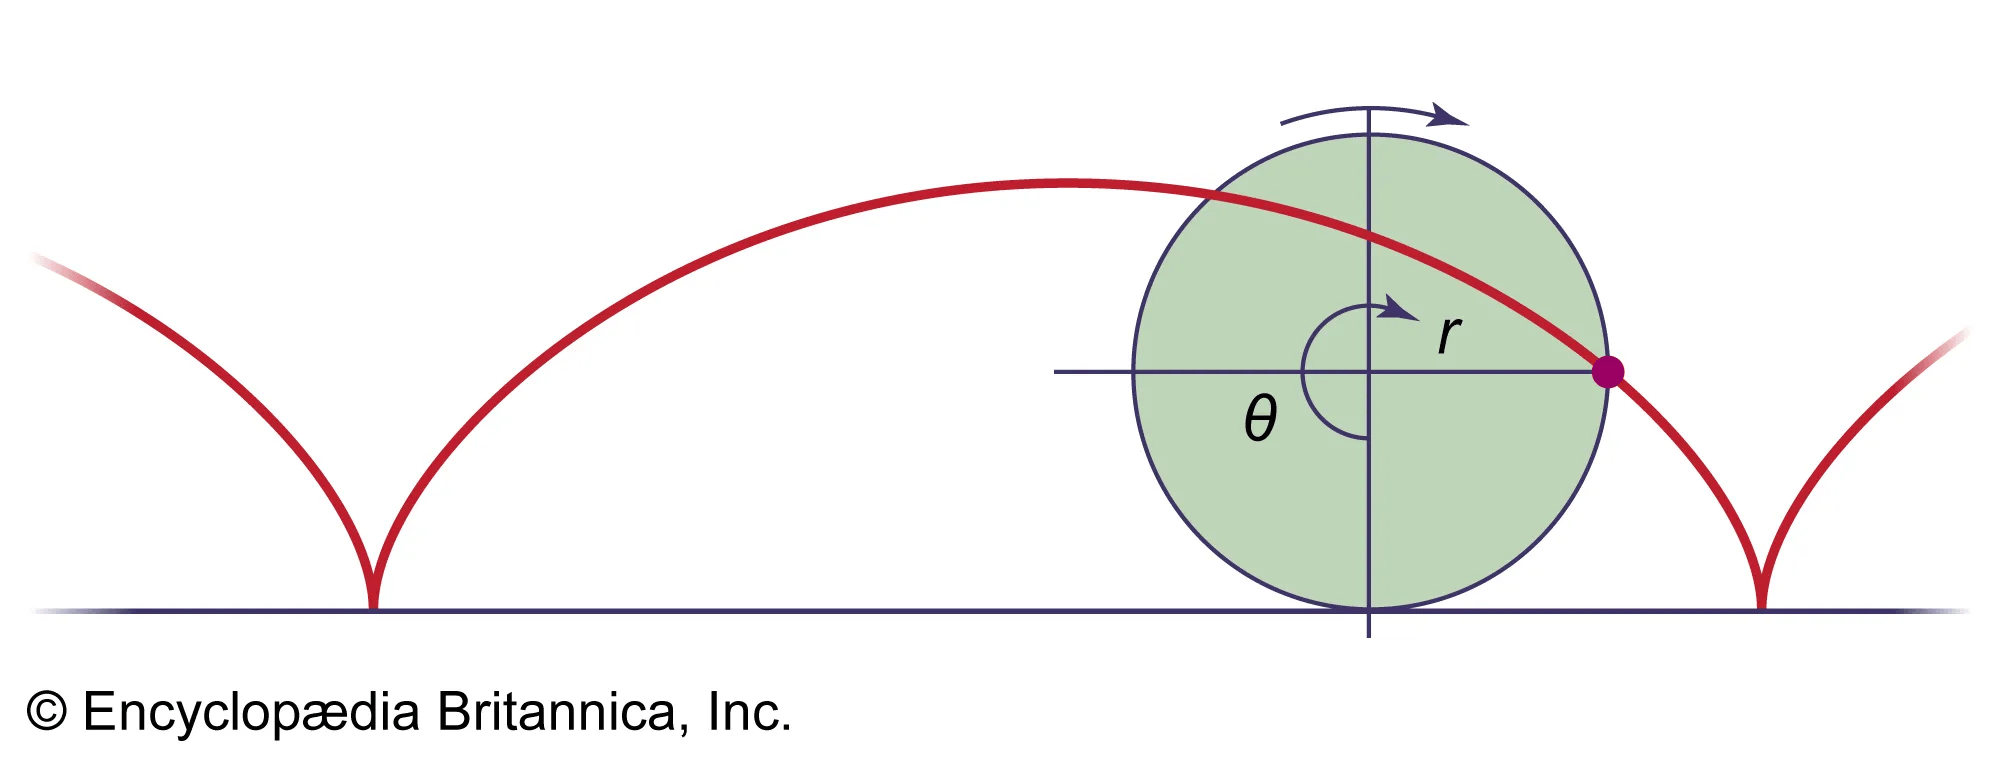
\includegraphics[width=0.7\textwidth]{figures/CycloidalCurveCreation.png}
  \caption{Cycloidal curve generation}
  \label{fig:cycloidal_curve}
\end{figure}

When a cycloidal curve is generated with the base being another circle, it generates either an epicycloidal curve or a hypocycloidal curve.
In the epicycloidal case, the curve is produced by tracing a cycloidal curve on the outside of a circle, while a hypocycloidal curve is produced by tracing a cycloidal curve on the inside of a circle.
The following 2 figures show a epicycloidal and hypocycloidal curve, respectively:
\begin{figure}[H]
  \centering
  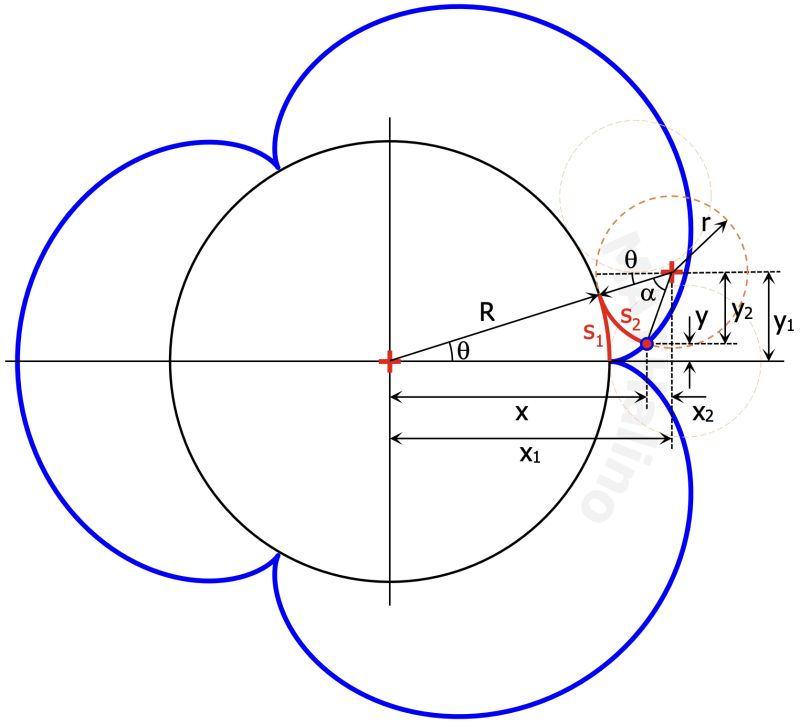
\includegraphics[width=0.7\textwidth]{figures/EpicycloidalCurve.png}
  \caption{Epicycloidal curve generation}
  \label{fig:epicycloidal_curve}
\end{figure}
\begin{figure}[H]
  \centering
  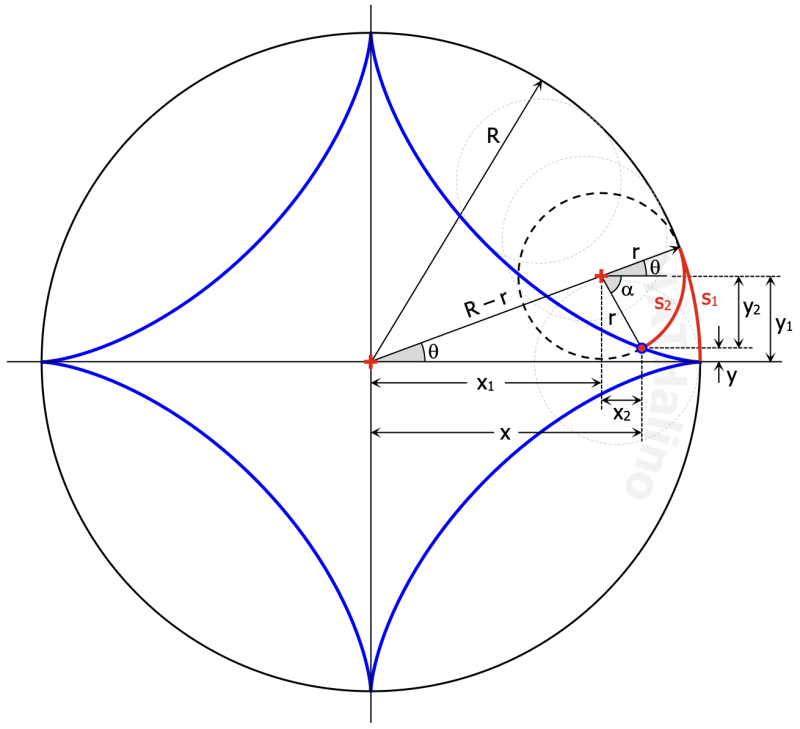
\includegraphics[width=0.7\textwidth]{figures/HypocycloidalCurve.jpg}
  \caption{Hypocycloidal curve generation}
  \label{fig:hypocycloidal_curve}
\end{figure}

A cycloidal curve is an easy to understand case of a trochoidal curve, which is the same as the cycloidal curve, except that the tracing point is not on the surface of the rolling circle, but is instead offset from the surface of the rolling circle by a distance $r$.
A hypotrochoidal curve and epitrochoidal curve are the trochoidal versions of hypocycloidal and epicycloidal curves.
This is shown in the following figure (note that a prolate curve is where the $r$ is greater than the tracing circle radius, while a curtate is where $r$ is less than the tracing circle radius):
\begin{figure}[H]
  \centering
  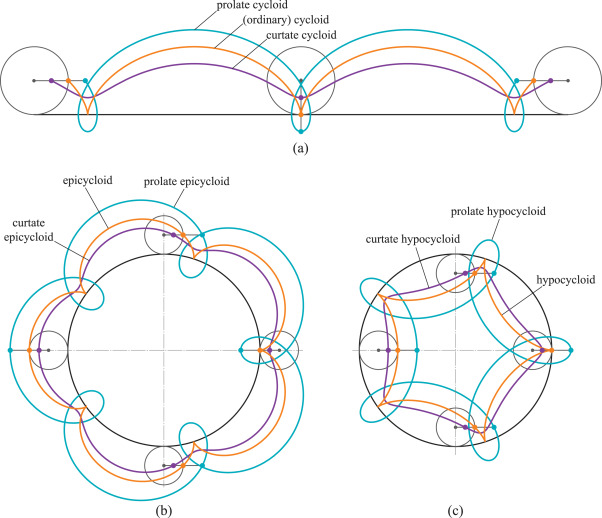
\includegraphics[width=0.6\textwidth]{figures/ProlateCurtateTrochoidCurves.jpg}
  \caption{Prolate and Curtate Trochoidal curves}
  \label{fig:trochoidal_curves}
\end{figure}
\newpage
Hypotrochoidal and epitrochoidal curves have a number of interesting properties:
\begin{itemize}
  \item The number of lobes, or segments, in the trochoid is the exact same as the ratio $k = \frac{R}{r}$, as labeled above in \ref{fig:trochoidal_curves}.
  \item The number of rotations of the tracing circle about its center for one full rotation around the base circle is $k + 1$ for epitrochoidal curves and $k - 1$ for hypotrochoidal curves.
  \item hypotrochoidal and epitrochoidal curves can be conjugates of one another and mesh together.
\end{itemize}

The second property can be used to reduce speed and convert to torque.

\subsection{Epitrochoidal Case}
In the epitrochoidal case, an inner disc is manufactured with an epitrochoidal profile.
It is eccentrically driven, and allowed to rotate about its own center.
The desirable outcome is a conjugate envelope for the epitrochoidal disc, which would allow for an even, rolling contact to achieve an effect the same as the hypocycloidal curve generation: a tracing circle orbiting inside a base circle.
Luckily, a hypotrochoidal envelope provides this desirable outcome.
By manufacturing an outer hypotrochoidal ring gear that has more lobes than the epitrochoidal disc


The kinematic relationship that is of interest is the number of revolutions done by the tracing circle to roll one full revolution around the base circle.
This is derived by Santos-Pereira in \cite{CycloidalGeometry}, and shows that for the epicycloid case, the number is:
\[
\frac{D}{d}+1
\]
and for the hypocycloid case:
\[
\frac{D}{d}-1
\]
where $D$ is the diameter of the base circle, and $d$ is the diameter of the tracing circle.
If $d$ becomes closer to $D$, the number of revolutions that the tracing circle does about its center becomes arbitrarily large for every one revolution around the base circle.
This angle relationship between the center revolutions of the tracing circle and the base circle forms the basis of the speed reduction in cycloidal drives.
For proper torque transmission, simple circles cannot be used for the mechanism, and instead meshing profiles are used between the tracing circle and base circle (for ease of understanding, cycloidal gear and ring gear will be used from now on).
\\\\
The cycloidal and ring gear teeth profiles may be involute, however only if there is a greater than 1 difference between the teeth count of the cycloidal and ring gear, ie $D - d > 1$.
This is due to interference issues with standard involute profiles if the difference is 1, and according to Jang et al, a comparison of involute and cycloidal profiles at this teeth ratio demonstrates that involute profiles have less rigidity and require major pressure angle adjustments to function \cite{InvoluteVsCycloidalComparison}.
\\\\
The general alternative to involute profiles is the pinwheel, -epitrochoid/hypotrochoid meshing. by replacing the ring gear with a set rollers which are equally spaced in a circle.
From the frame of reference of the cycloidal disc, the rollers trace an envelope around it as it eccentrically orbits. also naturally lends itself to the underlying principle of speed reduction used in this case. As demonstrated by Hwang and Hsieh in \cite{CycloidalKinematics}, "the cycloidal wheel profile will be produced using the inward equidistance to the extended epicycloid and the outward equidistance to the extended hypocycloid".
This is more easily seen in the following image:
\begin{figure}[H]
  \centering
  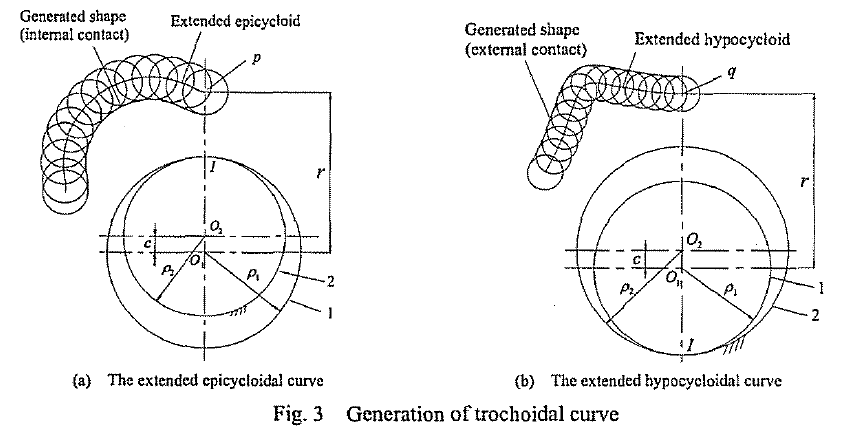
\includegraphics[width=0.8\textwidth]{figures/ExtendedTrochoidalCurveGeneration.png}
  \caption{Extended Epitrochoidal and Hypotrochoidal Curve Generation}
  \label{fig:extended_trochoidal_curve_generation}
\end{figure}
Meshing within

The key advantage of a cycloidal reducer is that the plate gear meshes at all points with the lobes, guaranteeing no backlash in a perfectly manufactured reducer, and the rolling contact between the plate gear and the lobes reduces wear and increases efficiency.

There are 4 different types of cycloidal speed reducer kinematic architectures
\cite{MechanismAndMachineTheoryPaper}:
\begin{itemize}
  \item The stationary ring gear type epicycloid reducer
  \item The rotating ring gear type epicycloid reducer
  \item The stationary ring gear type hypocycloid reducer
  \item The rotating ring gear type hypocycloid reducer
\end{itemize}

These can be broadly categorised between 2 aspects: epicycloidal or hypocycloidal profiles, and stationary or rotating ring gears.

\subsection{Practical Considerations}
.

\clearpage

\begin{thebibliography}{9}
  \bibitem{MechanismAndMachineTheoryPaper}
  Joong-Ho Shin, Soon-Man Kwon, On the lobe profile design in a cycloid reducer using instant velocity center, Mechanism and Machine Theory, Volume 41, Issue 5, 2006, Pages 596-616, ISSN 0094-114X, https://doi.org/10.1016/j.mechmachtheory.2005.08.001.
  \bibitem{CycloidalGeometry}
  Santos-Pereira, O. L., Ferreira, M. (Eds.) (2025). Roullete curves, coin paradox and aristotle's wheel paradox. Revista Brasileira de Ensino de Física. 47. https://doi.org/10.1590/1806-9126-RBEF-2025-0401.
  \bibitem{CycloidalKinematics}
  Hwang, Y.-W., Hsieh, C.-F. (2006), “Geometry design and analysis for trochoidal-type speed reducers: With conjugate envelopes,” Transactions of the Canadian Society for Mechanical Engineering, 30(2). DOI: 10.1139/tcsme-2006-0016.
  \bibitem{InvoluteVsCycloidalComparison}
  Dae-Jin Jang et al. (2021), “Geometry design and dynamic analysis of a modified cycloid reducer with epitrochoid tooth profile,” Mechanism and Machine Theory, 164, 104399.
\end{thebibliography}

\end{document}
